\chapter{Coherence Estimation}
\label{chap:coherence}


\section{Introduction}

A number of practical applications benefit of the knowledge about the diffuseness of a sound field, including speech enhancement and dereverberation \cite{p_habets_dual-microphone_2006}, noise suppression \cite{ito_designing_2010}, source separation \cite{duong_under-determined_2009} or background estimation \cite{stefanakis_foreground_2015}. In the field of spatial audio, diffuseness estimation is often used for parametrization \cite{pulkki2006directional, politis_compass_2018}, Direction-of-Arrival estimation \cite{thiergart_localization_2009} or source separation \cite{motlicek_real-time_2013}.

In this Chapter, we study diffuseness estimation by subjecting a tetrahedral microphone array to spherically isotropic noise fields.
The motivation for this work is, first, that tetrahedral arrays are a well known type of microphone arrays, which have today become popular for applications related to Virtual and Augmented Reality. 
Second, the spherical isotropic sound field is known to be a good approximation to the reverberant part of the sound field in a room \cite{elko_spatial_2001, mccowan_microphone_2003}, and therefore it would be interesting to investigate how different microphone arrays behave under such conditions.




\subsection{Problem definition}

Under spherical isotropic noise, the theoretical coherence between any pair of zeroth- and first-order ambisonic virtual microphones is equal to 0 for all frequencies, due to the spherical harmonic orthogonality (Eq.~\ref{eq:orthonormality}) \cite{elko_spatial_2001}. This result can also be assessed by Eq.~(\ref{eq:closedform_msc}).

However, there are several practical factors that might corrupt the coherence estimation, such as the approximation of the temporal expectation by time averaging \cite{thiergart_diffuseness_2011} in Eq.~(\ref{eq:psidefinition}), or the non-ideal implementation of the radial filters $\Gamma_n(kR)$ (Eq.~\ref{eq:a2b}) for the \textit{A-B conversion}\cite{schorkhuber_ambisonic_2017}.

In the following sections, we present several experiments that illustrate the behavior of different coherence estimators applied on the signals captured with a tetrahedral microphone subjected to spherical isotropic noise, using both simulated and real sound recordings.



\section{Methods}

\subsection{Simulation}
Spherical isotropic noise has been generated following the \textit{geometrical method} \cite{habets_generating_2007, habets_comments_2010}, using $I = 1024$ plane waves. The resulting \textit{A-Format} signals correspond to a virtual tetrahedral microphone array mimicking the Ambeo\footnote{Sennheiser Ambeo VR Mic \cite{sennheiser}.}
characteristics ($R=0.015$ meter, $\alpha=0.5$). 
The generated audio has a duration of 60 seconds. 





\subsection{Recording}

Spherical isotropic noise has been rendered to a spherical loudspeaker layout with 25 \textit{Genelec 8040}. The loudspeakers are arranged into three azimuth-equidistant 8-speaker rings at inclinations $\vartheta = [\pi/4, \pi/2, 3\pi/4]$, plus one speaker at the zenith.
The different speaker distances to the center are delay- and gain-corrected, and the signal feeds are equalized to compensate for speaker coloration. The room has an approximate $T_{60}$ of 300 ms measured at the 1 kHz third-band octave. 

The spherical isotropic noise has been also created by the \textit{geometrical method}, encoding a number of uncorrelated noise plane waves in ambisonics with varying orders $N \in [1,5]$. Due to practical limitations related with the software, the minimum number of sources $I = 256$ for an accurate sound field reconstruction \cite{habets_comments_2010} could not be reached - instead, the analysis has been performed parametrically with $I = [8, 16, 32, 64]$.
For each value of $N$ and $I$, approximately 15 seconds of audio have been recorded with an Ambeo microphone located at the center of the speaker array.

Ambisonics decoding is performed with an AllRAD decoder, passing through a spherical 64-point 10-design virtual speaker layout, and includes an imaginary speaker at the nadir. The decoding matrix uses \textit{in-phase} weights.



\subsection{Data processing and metrics}

The sampling rate of all signals is 48 kHz.
All frequency-domain results have been obtained by averaging their time-frequency representations over time.  
\textit{A-B conversion} has been computed using \textit{Ambeo A-B converter} AU plugin, version 1.2.1.

Two error metrics are considered: the frequency-dependent squared error $\varepsilon(k)$:
\begin{equation}
	\varepsilon(k) = |X_1(k) - X_2(k)|^2,
	\label{eq:mse}
\end{equation}

 and the mean squared error $\bar{\varepsilon}$:

\begin{equation}
    \bar{\varepsilon} = \frac{1}{K}{\sum_{k=1}^{K} |X_1(k) - X_2(k)|^2}
    \label{eq:nmse}
\end{equation}



\section{Results and discussion}
\subsection{\label{subsec:results_aformat}A-Format}



The coherence of the generated \textit{A-Format} signals is exemplified in Fig.~\ref{fig:Fig1} (left), which shows the $MSC$ between the capsule pair (\textit{BLD,BRU}) for the theoretical, simulated and recorded cases.
The theoretical coherence is derived from Eq.~(\ref{eq:closedform_msc}), while simulated and recorded MSC have been computed by Welch's method, using a \textit{hanning} window of 256 samples and 1/2 overlap.
The difference between theoretical and simulated coherence is negligible for practical applications.
However, there is a noticeable difference when compared to the recorded coherence. 
In general, the recorded $\text{MSC}$ follows the tendency of the simulated curve up to around 5 kHz.
Above this frequency, the recorded $MSC$ presents several spectral peaks, which might be partially explained by the interference of the microphone itself in the recorded sound field, and by the non-ideal directivity of the capsules.
The squared error $\varepsilon(k)$ with respect to the simulated curve is shown in Fig.~\ref{fig:Fig1} (left), while Fig.~\ref{fig:Fig1} (right) represents the same error averaged over frequency $\bar{\varepsilon}$ for different spatial resolution values of the diffuse field reproduction algorithm.
As expected, $\bar{\varepsilon}$ decreases with increasing values of $N$ and $I$.

\begin{figure}[th]
	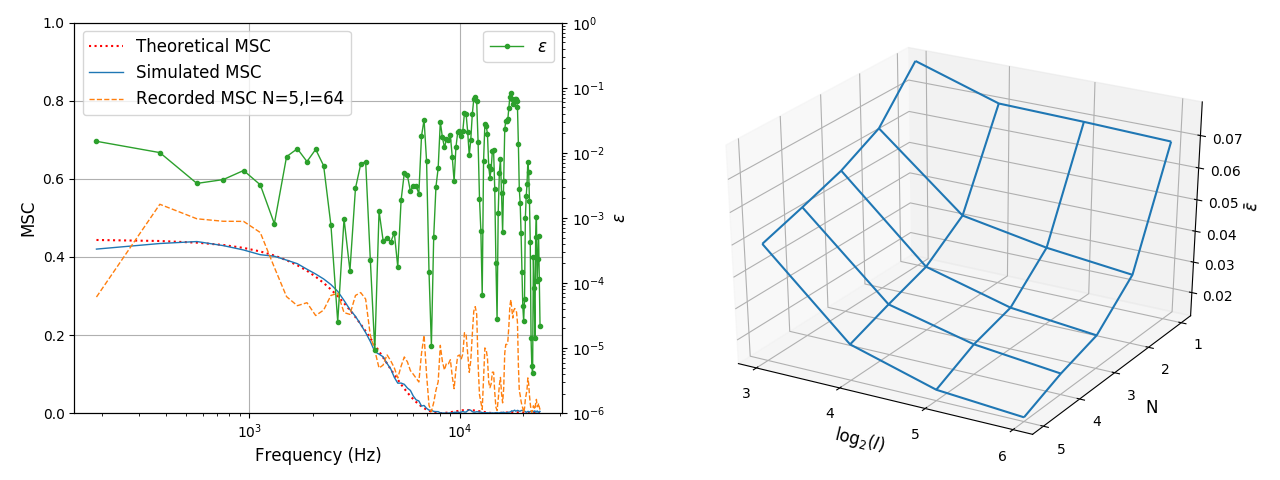
\includegraphics[width=\textwidth]{Figures/CoherenceEstimation/Untitled1}
    \caption{\label{fig:Fig1}\textit{A-Format} coherence between microphone signals. Left: $\text{MSC}$ as a function of the frequency of theoretical, simulated and recorded \textit{((BLD,BRU)},  $N=5, I=64$) signals. Right: mean error $\bar{\varepsilon}$ of the recorded signals' $MSC$ \textit{(BLD,BRU)} compared to the simulated values, for all values of $N$ and $I$.}
\end{figure}



\subsection{B-Format} 

In order to evaluate the dependency of the \textit{B-Format coherence} $\Delta$ on the number of time frames used for averaging, the following procedure is presented.
The simulated \textit{A-Format} sound field has been transformed into the spherical harmonic domain, with and without the application of radial filters $\Gamma_n(kR)$ (Eq.~\ref{eq:a2b}). Then, $\Delta$ has been computed with Eq.~(\ref{eq:delta}) for exponentially growing values of $r$ between 1 (8 ms) and 2048 (10.92 s), where $r$ is the vicinity radius used for time averaging, and the number of time windows is given by $T = 2r+1$.
The time-frequency representation is derived by applying the STFT with the same window parameters as in Subsection \ref{subsec:results_aformat}.\\

\begin{figure}
	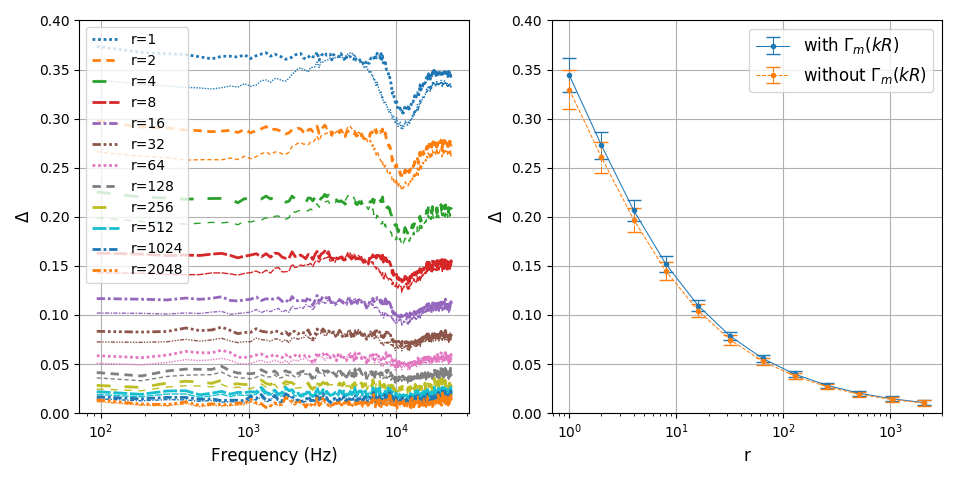
\includegraphics[width=\textwidth]{Figures/CoherenceEstimation/Figure2}
	\caption{\label{fig:Fig2} Estimated \textit{B-Format} coherence ($\Delta$) of a simulated diffuse sound field, as a function of the temporal averaging vicinity radius $r$. Left: $\Delta(k)$ for different values of $r$, with (coarse) and without (fine) application of radial filters. Right: mean and standard deviation of $\Delta(k)$ as a function of $r$.}
\end{figure}


Figure~\ref{fig:Fig2} (left) shows the great dependence of $\Delta$ on $r$.  The estimated coherence tends to the theoretical values with increasing values of $r$. This tendency is better appreciated in Fig.~\ref{fig:Fig2} (right): the curve asymptotically decreases to a value $\Delta_{min}\approx0$.

Another interesting observation comes from the frequency response of the curves. For all values of $r$, the coherence of the compensated \textit{B-Format} signal (with $\Gamma_m(kR)$) is roughly flat up to around 7 kHz, which approximately corresponds to the operational spatial frequency range of the microphone \cite{gerzon1975design}.
Above this value, the coherence response looses the flatness due to spatial aliasing (Eq.~\ref{eq:falias}). The response above the maximum frequency could be stabilized, if needed, by alternative diffuseness estimation methods \cite{politis_direction--arrival_2015}.

The coherence level differences along frequency are inversely proportional to $r$ --- the effect is better depicted by the standard deviation values (right).
The effect of the radial filters in the coherence measurement is also shown: for a given $r$, the shape of the coherence is always less flat if no filters are applied. Conversely, in this case, coherence values are always smaller for the same $r$. This effect might be explained taking into account the inter-channel coherence introduced by microphone and encoder imperfections in real scenarios \cite{schorkhuber_ambisonic_2017}.

As a remark, the comparison between Figs.~\ref{fig:Fig1} and \ref{fig:Fig2} provides evidence that the application of the spherical harmonic transform might be able to yield more accurate diffuseness estimations, due to a better signal conditioning \cite{epain2016spherical}.\\


\begin{figure}
	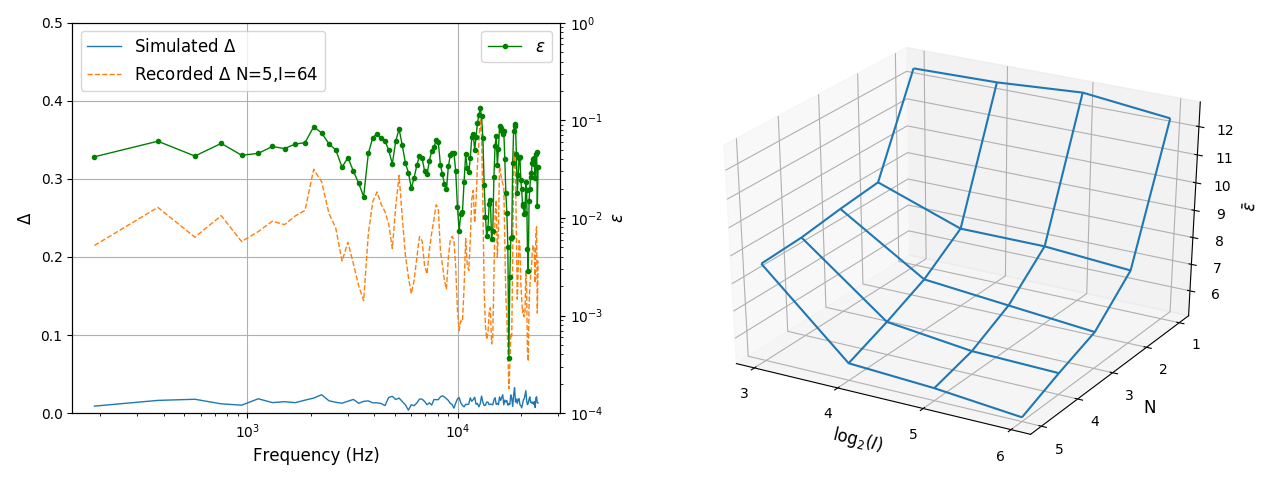
\includegraphics[width=\textwidth]{Figures/CoherenceEstimation/Untitled2}
	\caption{\label{fig:Fig3}\textit{B-Format coherence} between microphone signals. Left: $\Delta$ of simulated and recorded ($N=5, I=64$) signals. Right: $\bar{\varepsilon}$ of the recorded signals coherence across all values of $N$ and $I$.}
\end{figure}

Figure~\ref{fig:Fig3} (left) shows the estimated coherence for the recorded sound field with $N=5$ and $I=64$, using a vicinity radius of $r=1024$ ($\approx$ 5 s).
The curve is centred around $\Delta=0.25$ and presents several spectral peaks, as in the \textit{A-Format} case. 
It is important to notice here that the deviations between the coherence of the simulated and the recorded sound fields are much stronger compared to those of Fig.~\ref{fig:Fig1}. 

This effect can be also appreciated in Fig.~\ref{fig:Fig3} (right): the mean squared error is around two orders of magnitude higher in \textit{B-Format}.
Nevertheless, similar as in Fig.~\ref{fig:Fig1} (right), $\bar{\varepsilon}$ decreases with increasing values of $N$ and $I$.
This behavior suggests that the deviations between the recorded and the simulated coherence can be to a large degree explained by the low spatial resolution of the reproduction system; given a higher number of loudspeakers, we expect that the reproduced diffuseness will tend to the theoretical expression.




\section{Conclusions}
The diffuseness of a sound field is an important parameter for several applications. In this work, two different metrics of diffuseness have been defined and measured with a tetrahedral microphone subjected to spherical isotropic noise.

The analysis shows, first, the impact of the time-averaging window length on the \textit{B-Format} diffuseness estimator.
This result might be useful for designing coherence estimators that are parametrized with respect to the length of the analysis window \cite{thiergart_diffuseness_2011}.

Second, the feasibility of diffuse sound field reproduction by a spherical loudspeaker array using ambisonics plane-wave encoding and the \textit{geometrical method} is studied. 
Results suggest that this approach is viable, given a sufficient spatial resolution; a quantification of the impact of the number of loudspeakers remains for future work.




